%----------------------------------------------------------------------------------------
%	PACKAGES AND OTHER DOCUMENT CONFIGURATIONS
%----------------------------------------------------------------------------------------

\documentclass{article}

\usepackage{fancyhdr} % Required for custom headers
\usepackage{lastpage} % Required to determine the last page for the footer
\usepackage{extramarks} % Required for headers and footers
\usepackage[usenames,dvipsnames]{color} % Required for custom colors
\usepackage{graphicx} % Required to insert images
\usepackage{listings} % Required for insertion of code
\usepackage{courier} % Required for the courier font
\usepackage{lipsum} % Used for inserting dummy 'Lorem ipsum' text into the template
\usepackage{hyperref}

% Margins
\topmargin=-0.45in
\evensidemargin=0in
\oddsidemargin=0in
\textwidth=6.5in
\textheight=9.0in
\headsep=0.25in

\linespread{1.1} % Line spacing

% Set up the header and footer
\pagestyle{fancy}
%\lhead{\header} % Top left header
%\chead{\header} % Top center head
%\rhead{\firstxmark} % Top right header
\lfoot{\lastxmark} % Bottom left footer
\cfoot{} % Bottom center footer
%\rfoot{Page\ \thepage\ of\ \protect\pageref{LastPage}} % Bottom right footer
\rfoot{\thepage} % Bottom right footer
\renewcommand\headrulewidth{0.4pt} % Size of the header rule
\renewcommand\footrulewidth{0.4pt} % Size of the footer rule

\setlength\parindent{0pt} % Removes all indentation from paragraphs

%----------------------------------------------------------------------------------------
%	CODE INCLUSION CONFIGURATION
%----------------------------------------------------------------------------------------

\definecolor{MyDarkGreen}{rgb}{0.0,0.4,0.0} % This is the color used for comments
\lstloadlanguages{Perl} % Load Perl syntax for listings, for a list of other languages supported see: ftp://ftp.tex.ac.uk/tex-archive/macros/latex/contrib/listings/listings.pdf
\lstset{language=c++, % Use c++ in this example
        frame=single, % Single frame around code
        basicstyle=\footnotesize\ttfamily, % Use small true type font
        keywordstyle=[1]\color{Blue}\bf, % Perl functions bold and blue
        keywordstyle=[2]\color{Purple}, % Perl function arguments purple
        keywordstyle=[3]\color{Blue}\underbar, % Custom functions underlined and blue
        identifierstyle=, % Nothing special about identifiers                                         
        commentstyle=\usefont{T1}{pcr}{m}{sl}\color{MyDarkGreen}\footnotesize, % Comments small dark green courier font
        stringstyle=\color{Purple}, % Strings are purple
        showstringspaces=false, % Don't put marks in string spaces
        tabsize=4, % 4 spaces per tab
        %
        % Put standard Perl functions not included in the default language here
        morekeywords={rand},
        %
        % Put Perl function parameters here
        morekeywords=[2]{on, off, interp},
        %
        % Put user defined functions here
        morekeywords=[3]{test},
       	%
        morecomment=[l][\color{Blue}]{...}, % Line continuation (...) like blue comment
        numbers=left, % Line numbers on left
        firstnumber=1, % Line numbers start with line 1
        numberstyle=\tiny\color{Blue}, % Line numbers are blue and small
        stepnumber=5 % Line numbers go in steps of 5
}

% Creates a new command to include a perl script, the first parameter is the filename of the script (without .pl), the second parameter is the caption
\newcommand{\codescript}[2]{
\begin{itemize}
\item[]\lstinputlisting[caption=#2,label=#1]{#1.cpp}
\end{itemize}
}

\newcommand{\docscript}[2]{
\begin{itemize}
\item[]\lstinputlisting[caption=#2,label=#1]{#1}
\end{itemize}
}

\newcommand{\header}{TBM} % Course/class
\newcommand{\AuthorName}{Yuan-Yen Tai} % Your name

%----------------------------------------------------------------------------------------
%	TITLE PAGE
%----------------------------------------------------------------------------------------

\title{
\vspace{1in}
\textmd{\textbf{Tight Binding Model for Materials at Mesoscale: TBM$^3$}}\\
\vspace{1in}
}


\author{\textbf{\AuthorName}}
\date{} % Insert date here if you want it to appear below your name

%----------------------------------------------------------------------------------------

\begin{document}



\maketitle

\vspace{1in}
\begin{center}

\includegraphics[scale=0.3]{TBMCube-LOGO.pdf}
\end{center}

%----------------------------------------------------------------------------------------
%	TABLE OF CONTENTS
%----------------------------------------------------------------------------------------

%\setcounter{tocdepth}{1} % Uncomment this line if you don't want subsections listed in the ToC

\newpage
\tableofcontents
\newpage


\section{Introduction}

{\bf ``Tight Binding Model for Materials Mesoscale"} is a C++ based package and framework that designed for construct `any' kind of lattice structure with multi-orbital and spin degree of freedom to solve the basic nano-scale electronic structure.
Our goal is to construct a highly flexible and reusable framework for anyone to easily solve the multi-scale quantum mechnical model, $H^{tot} = H^0+ H^{int}$.

\begin{equation}
	\label{hopping}
	H^0 = \sum_{i\delta,\alpha\beta,s} t_{i,i+\delta,\alpha\beta}\, c^\dagger_{i,\alpha s} c_{i+\delta,\beta s}
\end{equation}

Listing.~\ref{code_example_001} shows a TBM$^{3}$ example code for implement the hopping term for the hopping term (Eq.~\ref{hopping}), where this example describes a 3D model for the itinerant $e_g$-electron of a transition-metal-oxide.
This example firstly add the chemical potential term to the Hamiltonian, and describe the multi-scal summation operation ($\sum_{ij,\alpha\beta,s}\cdots$) in the while-loop, and finally added each component of the Hopping parameter to the Hamiltonian.

\codescript{code_example_001}{Example for implement $H^0$}

Without the TBM$^{3}$ package, such a piece of code needs hundreds of lines of programming to be completed.
However, conveniency is not the only adventage of the package.
We implemented the GPU computation for the matrix operation for the Hamiltonian which can effectiently boost the calculation speed for large lattice size problem.

\section{Package setup and essentials}
TBM$^{3}$ is based C++ and python programming languages, therefore we need to pre install several library for C++ and python for our construction.

\subsection{C++: CUDA and MAGMA library}
The cuda library is used to operate the nVidia graphic processing unit (Installed on hellgirl).

The magma library is a GPU based linear algebra libary to boost the matrix operation.

\subsection{PYTHON: Numpy, matplotlib, vpython, wx}
We need these library to visualize the input/output file and calculated results.

\subsection{Setup the TBM$^3$ package}
TBM$^3$ can be downloaded from 
\href{https://www.dropbox.com/sh/h47v4wwdijj07fy/AAB1sdfAC5KkP-swoGVH6l6ha?dl=0}{{\color{blue} here}}.
Currently we are still in the {\it alpha-testing-stage} for the TBM$^3$ package development, therefore the link is limited only to our group member.
However, we will make it open source in the near future.

\codescript{code_example_002}{The folder structure of the package}

Listing.~\ref{code_example_002} shows the folder structure of the package.
The easiest way to compile someone's own code is:\\
$\bullet\;\; 1. $ set up the {\bf source/lift/bin/} for the system path.\\
$\bullet\;\; 2. $ modify the file {\bf source/lift/bin/m16hg} for the environmental setting.\\

\section{The structure of TBM$^{3}$}

\begin{center}
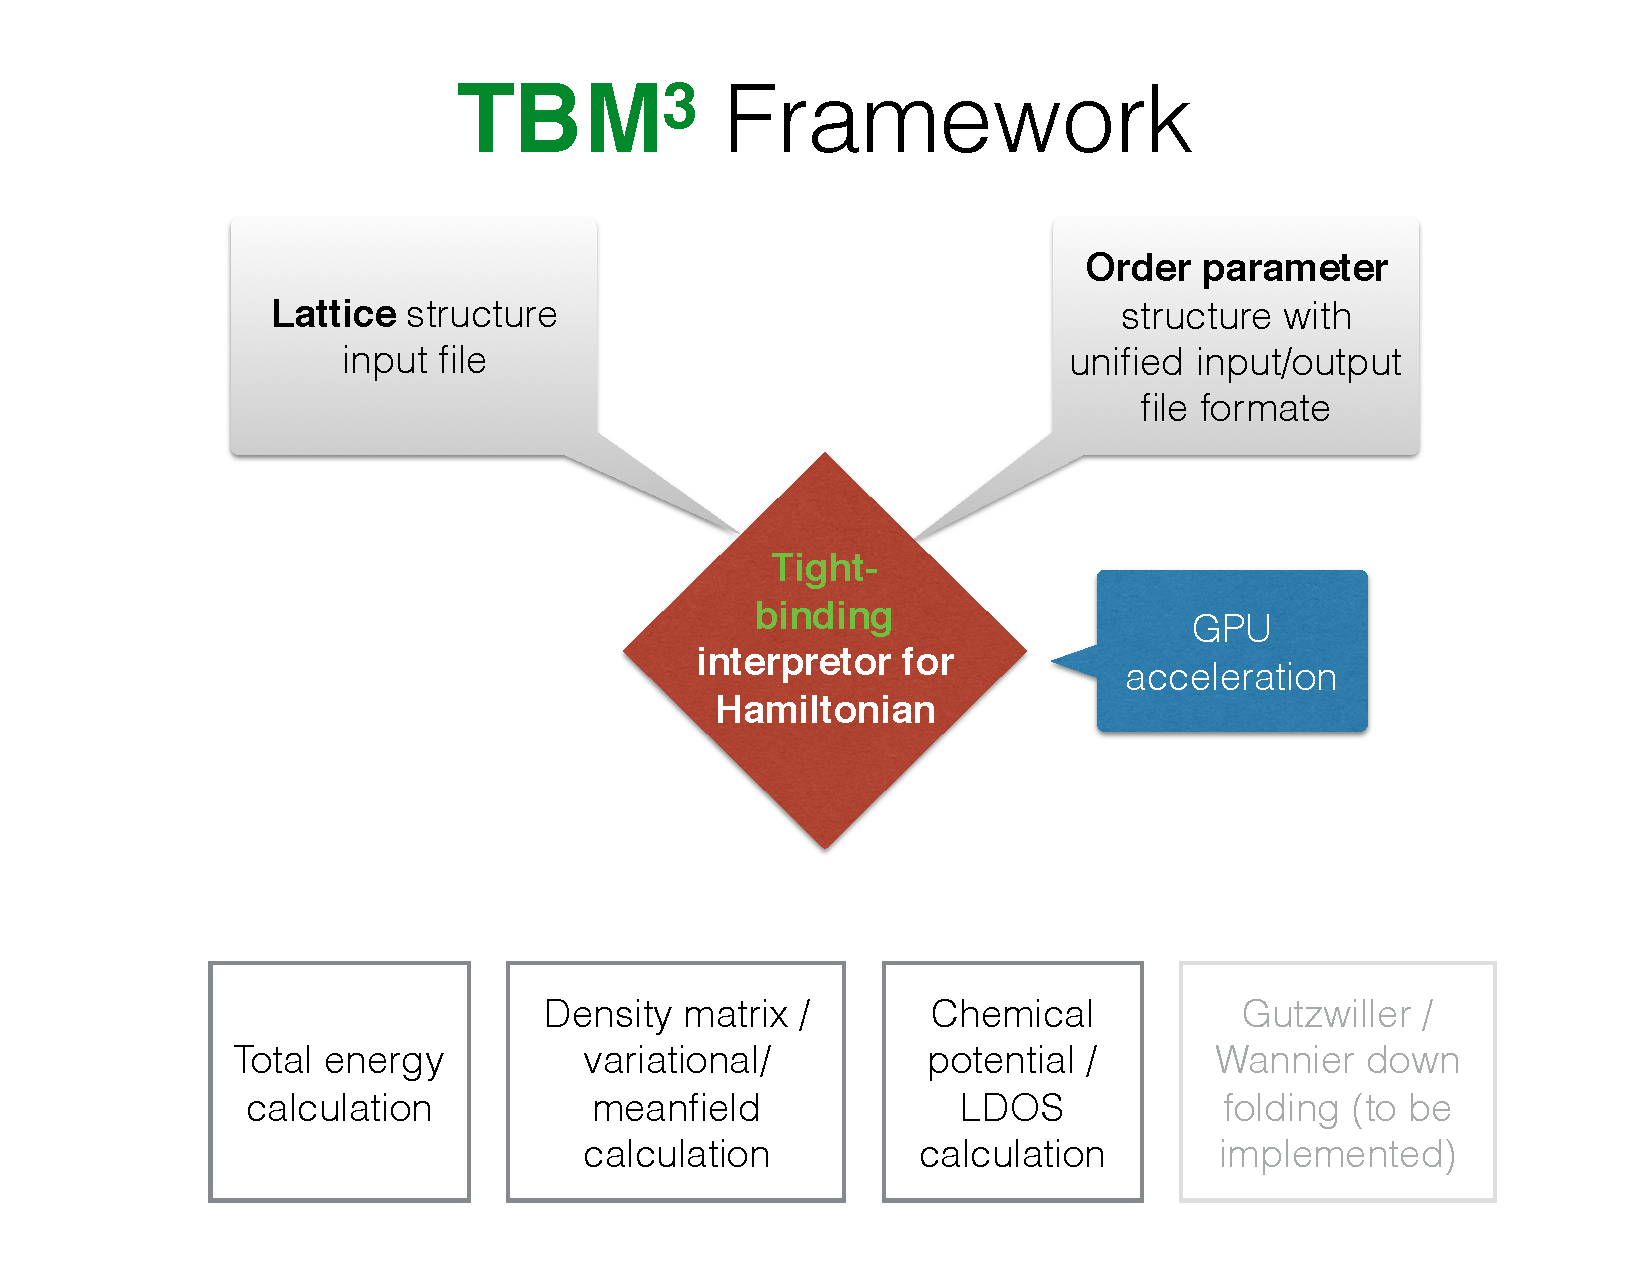
\includegraphics[scale=0.5]{fig01.pdf}
\end{center}

\section{Input file format}

The input file format contain several control blocks.\\
$\bullet 0.$ Parameters, which can construct any parameter to be used in the program.\\
$\bullet 1.$ Basis Vector, gives the dimension of the unitcell.\\
$\bullet 2.$ Sub Atoms, describe the position and orbital/spin degree of freedom.\\
$\bullet 3.$ Supercell Dim, makes it easy to construct repeated unitcell structure and convert into a large lattice structure.\\
$\bullet 4.$ Bonding basis, describe the smallest linking vector for each atom.\\
$\bullet 5.$ Bondings, describe the relations of all the atoms inside the lattice, periodic boundary condition is also considered.

The first thing to do with the input file is to use the `lift.py' script to check the formate and translate the file into a `.lif' file:\\
${\bf \$>:}$ {\bf lift.py filename.lat}\\
After doing this, the program will automatically generate a file `{\bf filename.lat.lif}' (if nothing wrong has been made), the input file is ready to be used for programming.

\docscript{00.Cubic.AFM.2x2x2.lat}{The input file format for a simple cubic structure}

Note that, after execute `lift.py filename.lat' the script automatically added two blocks into the input file:
$\bullet 7.$ Cell, describe all the atom informations in a supercell.\\
$\bullet 8.$ Neighbors, describe all the relations based on the inofrmation of $\bullet 4$, $\bullet 5$ and $\bullet 7$.\\

Once $\bullet 7$, $\bullet 8$ has been made, you can modify it such as change the atom name to make a hetero/interface structure.

\docscript{00.Cubic.AFM.2x2x2.lat.7-8}{The part after performing `lift.py filename.lat'}

You can use another python script to visualize the lattice structure and atom positions.\\
${\bf \$>:}$ {\bf vlift.py filename.lat}\\



\section{The programming structure}

In this section, I will show how to constructure the Hamiltonian and calculate the chemical potential, band structure, LDOS, total energy and LLG spin dynamics.
\begin{equation}
H = \sum_{i,j(=i+\delta),\alpha\beta,\sigma} t_{ij} c^\dagger_{i,\alpha,s} c_{j,\beta,s} - J_h\sum_{i\alpha} \vec \sigma_{i,\alpha} \cdot \vec S_i
\end{equation}

\codescript{code_example_003}{TBM$^3$ programming example}

\begin{center}
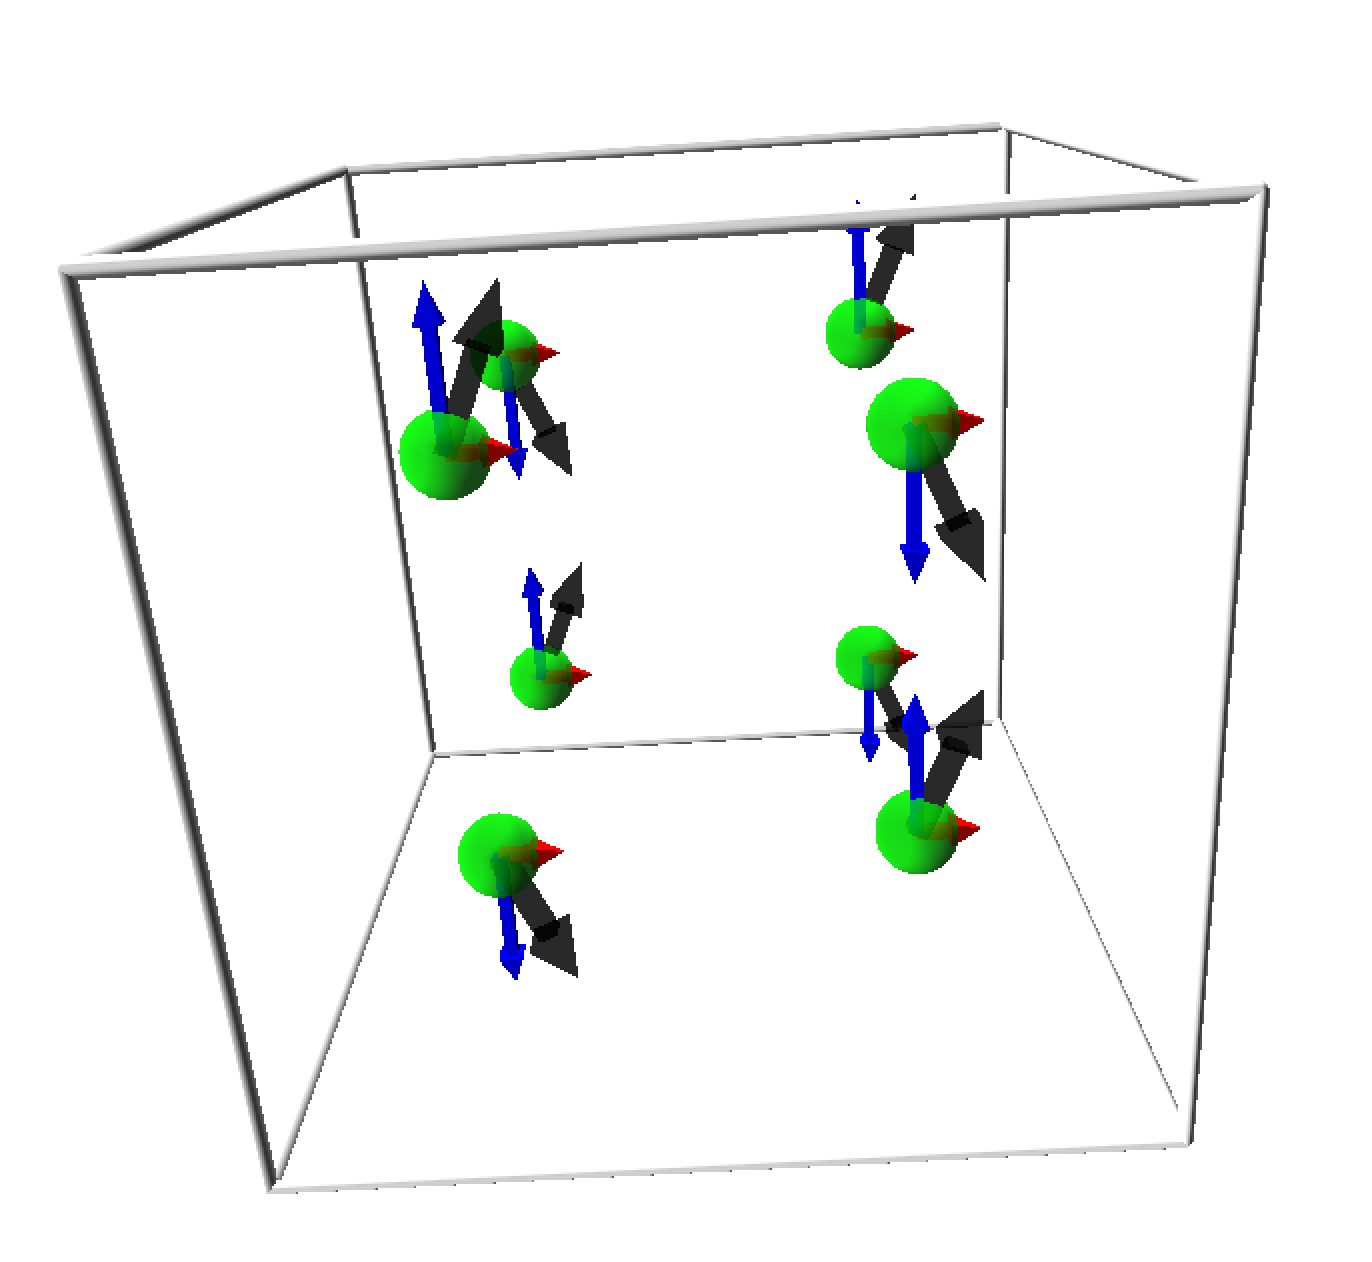
\includegraphics[scale=0.3]{fig02.png}
\end{center}
%
%
%\section{Implement the hopping parameter for lattice}


%----------------------------------------------------------------------------------------

\end{document}
